\subsubsection{\stid{1.07} Exascale MPI} \label{subsubsect:mpich}
\paragraph{Overview}

MPI has been the de facto standard programming model for HPC from the
mid 90's till today, a period where supercomputing performance
increased by six orders of magnitude.  The vast majority of DOE's
parallel scientific applications running on the largest HPC systems
use MPI. These application codes represent billions of dollars of
investment. Therefore, MPI must evolve to run as efficiently as
possible on Exascale systems. Our group at Argonne developed a
high-performance, production-quality MPI implementation, called MPICH.
The focus areas of the Exascale MPI / MPICH project are: (1)
continuous improvement of the performance and capabilities of the
MPICH software to meet the demands of ECP and other broader DOE
applications, (2) coordinate vendor and supercomputing center
interactions to ensure efficient solutions to applications, and (3) be
involved in the MPI forum and standardization efforts to ensure
continuity of the work beyond this project.

MPICH team is involved in the formation of the MPI Forum and have been
deeply involved in defining the MPI standard since 1992. MPICH has
helped prototype and define the majority of the features in the MPI
standard. As such, MPICH has been one of the most influential pieces of
software in accelerating the adoption of the MPI standard by the HPC
community. MPICH has been adopted by leading vendors into their own
derivative implementations. Examples include Intel (for Intel MPI), Cray
(for Cray MPI), IBM (for IBM PE MPI), Mellanox (for MLNX-MPI), Microsoft
(for MS-MPI), and Ohio State University (for MVAPICH). MPICH and its
derivatives are exclusively used in 7 of the top 10 supercomputers in
the world today. MPICH is the recipient of a number of awards including
an R\&D 100 award.

\paragraph{Key Challenges}

While we believe MPI is a viable programming model at Exascale, both
the MPI standard and MPI implementations have to address the
challenges posed by the increased scale, performance characteristics
and evolving architectural features expected in Exascale systems, as
well as the capabilities and requirements of applications targeted at
these systems. The key challenges are:

\begin{enumerate}

\item Interoperability with intranode programming models having a high
  thread count~\cite{Hybrid1, Hybrid2, FT2} (such as OpenMP,
  OpenACC and emerging asynchronous task models);

\item Scalability and performance over complex
  architectures~\cite{Perf1, Perf2, FT2, Perf4} (including high core
  counts, processor heterogeneity and heterogeneous memory);

\item Software overheads that are exacerbated by lightweight cores and
  low-latency networks;

\item Enhanced functionality (extensions to the MPI standard) based on
  experience with applications and high-level libraries/frameworks
  targeted at Exascale; and

\item Topics that become more significant as we move to the next
  generation of HPC architectures: memory usage, power, and
  resilience.

\end{enumerate}

\paragraph{Solution Strategy}

The Exascale MPI project has the following primary technical thrusts:
(1) \textbf{Performance and Scalability} (2) \textbf{Heterogeneity}
(3) \textbf{Topology Awareness} (4) \textbf{Fault Tolerance} and (5)
\textbf{MPI+X Hybrid Programming}.

Our solution strategy started by addressing performance and
scalability aspects in MPICH related to network address
management~\cite{memscal}.  Apart from this, we also looked at
communication strategies which allow the MPI library to be as
lightweight as possible~\cite{ch41, ch42}. Other solutions include
investigation and evaluation of communication relaxation hints,
investigation of optimizations to memory scalability in MPICH and
improvements to MPI RMA operations.

Exascale MPI heterogeneity efforts~\cite{Hetero1, Hetero2, Hetero3}
started with the survey on heterogeneous memory architectures on
upcoming DOE machines and how MPICH can take advantage of
them~\cite{hexe}. The efforts also included the investigation of
utilizing heterogeneous memory inside the MPI implementation and
evaluation of applications~\cite{hetero4}. The heterogeneity efforts
further extended to investigating and developing technologies for GPU
integration for the better support of the coming Exascale
supercomputers.

Exascale MPI topology awareness efforts~\cite{Topo1,Topo2} originated
with the investigation and evaluation of hints based on topology
awareness and optimizations to virtual topology functionality in
MPICH~\cite{topo-io,topo-io2}. The other efforts include investigation
of topology-aware collectives and neighborhood collectives in
MPICH~\cite{coll} and evaluation of the selected ECP applications.

Exascale MPI fault tolerance efforts~\cite{FT1, FT2} started with
support for handling noncatastrophic errors in MPI. The second effort
included defining the scope of errors in MPI, a prerequisite for
user-level failure mitigation. Other efforts in this direction
includes standardizing these efforts in MPI and evaluating application
suitability for fault tolerance.

Exascale MPI+X hybrid programming developed firstly with effort in
improving interoperation of MPICH with threads~\cite{interthread}.
Secondly, we developed the work-queue data transfer model for
multithreaded MPI communication~\cite{workq}. We have included support
for interaction of MPICH with user-level thread (ULT)
libraries~\cite{ULT}, primarily targeting Argobots and the BOLT
runtime~\cite{BOLT}.  Other issues that are being looked at include the
investigation and evaluation on multiple virtual communication
interfaces for multithreaded MPI communication~\cite{VCI}.

\paragraph{Recent Progress}

One major achievement of MPICH recently is the support for the newly
released MPI-4 standard. The MPI-4 standard introduced new ways for
communication including persistent collective that aims to reduce the
overhead of repetitively setting up colllective, and partitioned
communication which aims to improve the performance for multi-threaded
MPI communication. The MPICH 4.0a1 release has include all the MPI-4 new
features.

Validation and verification has been an integral part of MPICH project.
We have made several improvements to the automated testing
infrastructure for more effective testing. We have also setup continuous
integration (CI) service with the ECP CI server and use it to test MPICH
on pre-exascale systems. This allows us to validate and verify MPICH
with different hardward configuration. Through these new testing
infrastructures, we have identified new issues which leads to
optimizations that improves the MPICH performance on pre-exascale
systems.

Lastly, we focus on better GPU support in MPICH. MPICH is now support
GPUs from all three vendors (NVIDIA, AMD and Intel). The support for
GPU communication include a fast path that utilizes the hardware RDMA
support for GPU memory, and a fallback path for cases like complex
datatypes which can not be directly handed by hardware RDMA. We have
also developed prototypes for GPU-stream-triggered operation. It allows
MPI application to enqueue MPI point-to-point communication to a GPU
stream or command queue. This allows the GPU stream to be used to manage
the synchronization between GPU kernels and the MPI communication that
depends on the result of those kernels. The benefit includes better
overlapping between computation and communication, and higher GPU
utilization.

\begin{figure}[htb]
  \centering
  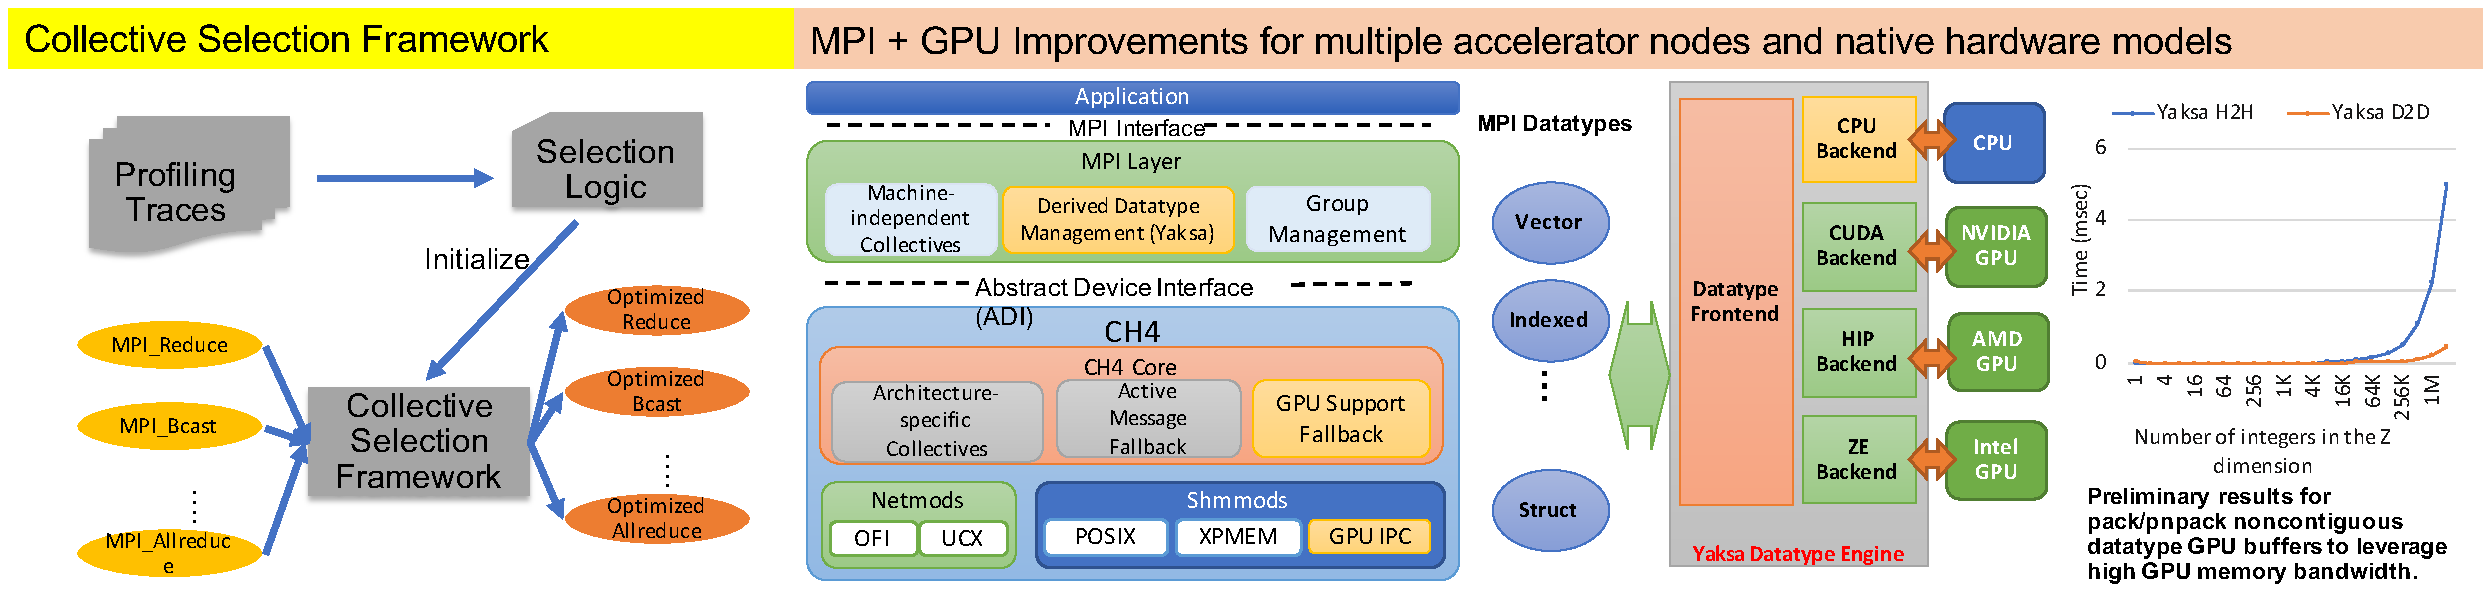
\includegraphics[width=6in]{projects/2.3.1-PMR/2.3.1.07-Exascale-MPI/MPICH-recent-milestones.pdf}
  \caption{\label{fig:fy20}Major MPICH milestones completed in fiscal year 2020}
\end{figure}

\paragraph{Next Steps}
In the next year, we are going to keep optimizing the GPU support in
MPICH. Plan work includes performance evaluation and improvement on GPU
communication, support for GPU collectives, and the extending
GPU-stream-triggered operation to more MPI communication functions.
We will also expand the software validation and verification work on
pre-exascale and exascle system to make MPICH perform well on the target
machines.
